\documentclass[border=4pt]{standalone}
% Shared typography and colours for the standalone figures.
\usepackage{unicode-math}
\setmainfont{TeX Gyre Heros}
\setmathfont{TeX Gyre Pagella Math}
\usepackage{tikz}
\usetikzlibrary{arrows.meta,positioning,calc,decorations.pathreplacing}
\usepackage{pgfplots}
\pgfplotsset{compat=1.18}

% One colour per element or subsystem. Record the mapping in
% the working repository conventions and use it identically in every figure.
\definecolor{elemA}{HTML}{1F5FA8}
\definecolor{elemB}{HTML}{B8461B}
\definecolor{elemC}{HTML}{2E7D32}
\definecolor{elemD}{HTML}{6A4C93}
\definecolor{frameline}{HTML}{555555}

\begin{document}
\hyphenpenalty=10000
\exhyphenpenalty=10000
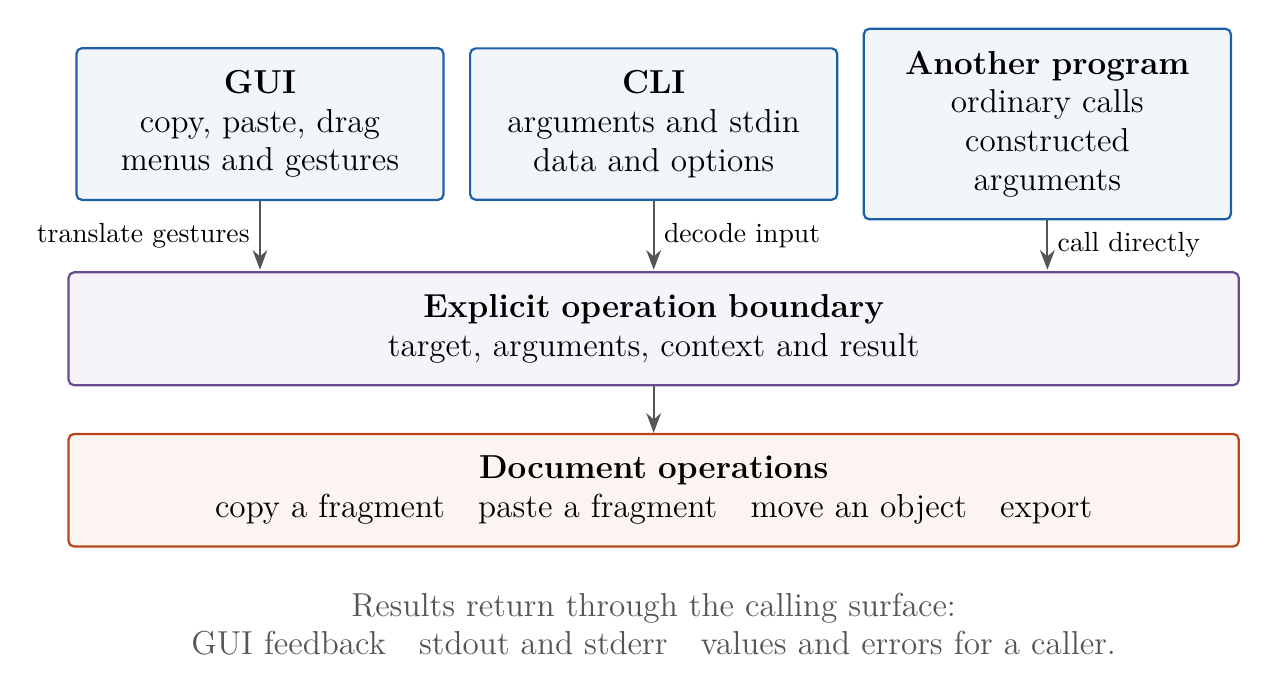
\begin{tikzpicture}[
  box/.style={draw,rounded corners=2pt,thick,align=center,inner sep=8pt,font=\large},
  surface/.style={box,draw=elemA,fill=elemA!6,text width=4.1cm,minimum height=1.8cm},
  arrow/.style={-{Stealth[length=2.5mm]},thick,draw=frameline}
]
\node[surface] (gui) at (-5,2.5) {\textbf{GUI}\\copy, paste, drag\\menus and gestures};
\node[surface] (cli) at (0,2.5) {\textbf{CLI}\\arguments and stdin\\data and options};
\node[surface] (app) at (5,2.5) {\textbf{Another program}\\ordinary calls\\constructed arguments};
\node[box,draw=elemD,fill=elemD!6,text width=14.3cm,minimum height=1.15cm] (boundary) at (0,-0.1)
  {\textbf{Explicit operation boundary}\\target, arguments, context and result};
\draw[arrow] (gui.south) -- node[left,font=\normalsize] {translate gestures} (-5,0.65);
\draw[arrow] (cli.south) -- node[right,font=\normalsize] {decode input} (0,0.65);
\draw[arrow] (app.south) -- node[right,font=\normalsize] {call directly} (5,0.65);
\node[box,draw=elemB,fill=elemB!6,text width=14.3cm,minimum height=1.2cm] (domain) at (0,-2.15)
  {\textbf{Document operations}\\copy a fragment\quad paste a fragment\quad move an object\quad export};
\draw[arrow] (boundary.south) -- (domain.north);
\node[align=center,text=frameline,font=\large,text width=14.4cm] at (0,-3.85)
  {Results return through the calling surface:\\GUI feedback\quad stdout and stderr\quad values and errors for a caller.};
\end{tikzpicture}
\end{document}
